\chapter{Hierarchical State Machines}\label{automata}

\statecharts~\cite{statecharts}\index{Statecharts} is a well used visual formalism for
hierarchical state machines which recently became the notation for
presenting behaviour in UML. There has been some dispute about its
semantics.  We use the synchronous semantics of
\synccharts~\cite{synccharts}\index{SyncCharts} that coincides with that given earlier
to \argos~\cite{argos}. 

However, though we share the view that the synchronous semantics has 
its benefits, a minor trick allows us to extend the synchronous 
semantics to capture the original \textsc{Statemate} semantics of 
\statecharts: we introduce a particular kind of delayed signals 
that, if emitted at one instant, become present only at the next 
instant.


\section{States and Preemption}

\paragraph{States as processes.}
\index{state!as process} Automata is
another familiar paradigm for both, engineers and computer
programmers.  Automata have states and transitions between these.  A
faintly new idea is to consider \emph{states as processes}.  A state may be
\emph{active} or \emph{inactive} as is the corresponding process.  The
process is started when a state is entered, it is active as long as
the automaton is in that state, and it is preempted when the state is
left.  For example, the behaviour of
\begin{center}
    {\tt\small
      \thinlines
      \setlength{\unitlength}{0.7pt}
      \begin{picture}(305,50)
          \put(100,30){\footnotesize when (?a) \{emit x\}}
           \put(87,25){\vector(1,0){145}}
           \put(0,0){
               \begin{picture}(80,50)
                    \put(0,38){\line(1,0){80}}
                    \put(0,0){\framebox(80,50){}}
                    \put(36,18){$P_{1}$}
                    \put(4,41){\scriptsize state1}
               \end{picture}
           }
           \put(225,0){
                \begin{picture}(80,50)
                     \put(4,41){\scriptsize state2}
                     \put(0,0){\framebox(80,50){}}
                     \put(36,18){$P_{2}$}
                     \put(0,38){\line(1,0){80}}
                 \end{picture}
           }
       \end{picture}
    }
\end{center}
is this: assume that the process $P_{1}$ is running if control is
in \pp{state1}.  This process is preempted if the signal \pp{a} is
present, the signal \pp{x} is emitted, and, at the same instant,
control passes to \pp{state2}, and the corresponding process $P_{2}$
is started.

In this interpretation, automata are just another notation for
structuring processes.  The implicit recursive definition justifies to
speak of \emph{hierarchical automata}\index{automaton!hierarchical}\index{automaton}; the process of a state can be
again specified by an automaton.  Obviously, any other specification
of a process in terms of the any of other language constructs
introduced so far might do as well.

\paragraph{Visual versus textual.}\index{automaton!textual}\index{automaton!visual} A visual presentation is attractive
if you deal with a customer.  For a programmer, textual notation may
be more condensed and more easily modified.  Here is the same example
in visual and textual presentation.
% 
\begin{center}
 {\tt\scriptsize    
 \setlength{\unitlength}{1.0pt}
  \begin{picture}(320,140)
    \thinlines
      \put(20,0){\begin{picture}(300,140)
      \put(-19,96){\circle{8}}
      \put(-16,93){\vector(2,-1){16}}
      \put(0,55){\begin{picture}(30,30)
       \put(4,22){off}
       \put(0,0){\framebox(30,30){}}
       \put(0,19){\line(1,0){30}}
       \end{picture}}
       \put(30,54){\bezier{100}(0,0)(25,-30)(75,-30)}
       \put(37,48){\vector(-1,1){7}}
       \put(30,85){\bezier{100}(0,0)(25,30)(75,30)}
       \put(101,115){\vector(1,0){5}}

     {\scriptsize
        \put(25,120){when (?start) \{\}}
        \put(-12,15){when (?stop | ?reset)}
        \put(-7,7){\{emit is\_elapsed;\}}
     }
    \put(100,0){
       \begin{picture}(180,140)
       \put(4,132){on}
        \put(0,0){\framebox(180,140){}}
       \put(0,129){\line(1,0){180}}

       \put(15,64){\begin{picture}(140,80)
       {\scriptsize
          \put(0,50){\circle{7}}
          \put(3,48){\vector(2,-1){16}}
          \put(20,15){\begin{picture}(25,25)
           \put(2,18){\tiny down1}
           \put(0,0){\framebox(25,25){}}
           \put(0,16){\line(1,0){25}}
           \end{picture}}
            \put(45,35){\vector(1,0){75}}
            \put(60,40){\tiny when (?incr)}
            \put(120,25){\vector(-1,0){75}}
            \put(55,15){\tiny when (?incr)}
            \put(60,5){\tiny \{emit carry;\}}
            \put(120,15){\begin{picture}(25,25)
            \put(2,18){\tiny up1}
           \put(0,0){\framebox(25,25){}}
           \put(0,16){\line(1,0){25}}
         \end{picture}}}
      \end{picture}}

       \put(0,64){\line(1,0){180}}

       \put(15,0){\begin{picture}(140,80)
       {\scriptsize
          \put(0,50){\circle{7}}
          \put(3,48){\vector(2,-1){16}}
          \put(20,15){\begin{picture}(25,25)
           \put(2,18){\tiny down2}
           \put(0,0){\framebox(25,25){}}
           \put(0,16){\line(1,0){25}}
         \end{picture}}
             \put(45,35){\vector(1,0){75}}
            \put(60,40){\tiny when (?carry)}
            \put(120,25){\vector(-1,0){75}}
            \put(55,15){\tiny when (?carry)}
            \put(60,5){\tiny \{emit reset;\}}
            \put(120,15){\begin{picture}(25,25)
           \put(2,18){\tiny up2}
           \put(0,0){\framebox(25,25){}}
           \put(0,16){\line(1,0){25}}
         \end{picture}}}
      \end{picture}}

    \end{picture}}
   \end{picture}}
  \end{picture}}
\end{center}
Here is the textual representation:
% 
\codeinput{four-bit-automaton}
% 
The automaton has two states \pp{off} and \pp{on}.  The \pp{init}
statement is \emph{instantaneous}, that is, it terminates in the same
instant it is started.  Hence, if the process/automaton is started it
moves on to the state \pp{off} and starts the process \pp{halt}.  In
\se, automata have initial transitions rather than initial states. 
The equivalent in the visual notation is a transition with a blob
rather than a state in its source.

A state can be left only when the condition of some outgoing
transition becomes true, but a state can be left only in the next
instant after it has been activated or after the next instant.  This mean
that a state is ``active'' for at least one instant.\footnote{In that preemption is delayed (cf. Section~\ref{reactive-control}).}  The process of
the state \pp{off} is specified by the statement \pp{do \{ nothing \}}
which does nothing (hence the statement may be omitted for
convenience).  Via the statement \pp{do \{$P$\}} any process $P$ can
be embedded.

If the \pp{start} signal is present in the next instant or later,
the automaton moves to state \pp{on}, and starts two processes, again
presented by automata. \pp{when ?start \{ next state on\}} is the
textual phrase for the transition with obvious connotation.

\paragraph{Preemption by a transition is weak.}\index{preemption!weak!for automata}
Rather than to carry on, we focus on the particular situation when the
automaton is in state \pp{on}, the subautomata are in state \pp{up1}
resp.  \pp{up2} and the signal \pp{incr} is present.  Then the first
subautomaton performs the transition and emits \pp{carry}.  At the
same instant, the other subautomaton performs its transition as well
since the signal \pp{carry} is present, and emits \pp{reset}.  Still
at the same instant, the process of state \pp{on} is preempted, and
the automaton moves to state \pp{off} emitting \pp{is\_elapsed}.  Note
that, though the actions of the transitions are executed, the
subautomata do not change state to \pp{down1} resp. \pp{down2}
due to preemption of state \pp{on}.

Preemption must be \emph{weak} in that the process of state \pp{on}
must be allowed to do all its computation in this instant, otherwise
the signal \pp{reset} will not be emitted.  Preemption takes place
from the inside, which would be impossible if preemption would be
strong.  Note further that the process can be preempted from the
outside by the signal \pp{stop}.

\section{Textual Presentation}\index{automaton!textual}
% \paragraph{Textual presentation.}
\index{Automata,textual syntax} The
textual syntax for automata is very simple.  The keyword
%
\BEP
automaton \{ $P$ \};
\EEP
%
indicates that the process $P$ is presented by an automaton.  The
specification of a \emph{state}\index{State,textual presentation} is
of the form
%
\BEP
state \textit{name}
    [ do     \{ $P$ \} ]
    [ entry  \{ $P_{entry}$ \} ]
    [ during \{ $P_{during}$ \} ]
    [ exit   \{ $P_{exit}$ \} ]
           when $C_{1}$ \{ $P_{1}$ \}
    [ else when $C_{2}$ \{ $P_{2}$ \} ]
    \ldots
    [ else when $C_{n}$ \{ $P_{n}$ \} ];
\EEP
%
All the clauses in square brackets are optional.  It is required that all
processes except for $P$ are instantaneous.
 \footnote{The pattern for is similar to that for preemption operators.
 This is not by chance. In 
% the formal semantics (cf.  Section
% \ref{semantics}) as well as in 
 the implementation there is a unique
 preemption operator used for all these cases.}

The behaviour is as follows.  When entering a state the processes $P$
and $P_{entry}$ are started.  The processes $P$ and $P_{during}$ are
active as long as the state is active.  When a condition $C_{i}$
becomes true, the process $P$ is weakly preempted and the process
$P_{exit}$. Finally the process  $P_{i}$ are started when $P_{exit}$
terminates. 
 At each instant, the
process $P$ executes before checking the conditions $C_{i}$ that are
checked in the obvious order.

The \emph{initial transition}\index{Transition,initial} has a similar
format
%
\BEP
init \{$P$\}
\EEP
%
with $P$ being instantaneous.

Finally, the statement
%
\BEP
next state \textit{state\_name};
\EEP
%
denotes the (instantaneous) jump to the next state. A particular form of the statement is the {\em next state exit}\index{next state,exit} statement
%
\BEP
next state exit;
\EEP
%
If this process is started the respective automaton terminates instantaneously. 

\section{Visual Presentation}\label{visual}\index{automaton!visual}

The visual syntax\index{Automata,visual syntax} is close to that of
\statecharts~\cite{statecharts} \index{Statecharts} and
\textsc{SyncCharts}~\cite{synccharts}\index{SyncCharts}.  Automata
have nodes and transitions.  Nodes are either persistent states or
transient states.  \emph{Transient states}\index{State,transient} of
the form of a circle are used for initial and terminal transitions,
and for conditionals.

\emph{Persistent states}\index{state!persistent} are of the form
\begin{center}
    {\tt\footnotesize  
     \setlength{\unitlength}{0.6pt}
    \begin{picture}(200,100)
     \put(0,0){\framebox(200,100){}}
    \put(4,90){\textit{name}} 
    \put(100,90){entry}
    \put(150,90){$P_{entry}$}
    \put(100,75){during}
    \put(150,75){$P_{during}$}
    \put(100,60){exit}
    \put(150,60){$P_{exit}$}
    \put(0,55){\line(1,0){200}}
    \put(918,25){$P$}
    \end{picture}}
\end{center}
The same conditions apply as for the obvious textual equivalent. The
body $P$ of a visual state is (at present) restricted to a few
formats (the restrictions apply recursively):
\begin{itemize}
    \item  the \emph{parallel operator} indicated by horizontal or
    vertical lines (\emph{and-states}\index{state!and state} in the terminology of
    statecharts)
    \begin{center}
    {\tt\footnotesize 
      \setlength{\unitlength}{0.6pt}
    \begin{picture}(160,70)
     \put(0,0){\framebox(160,70){}}
    \put(5,60){\textit{state}}
    \put(0,55){\line(1,0){160}}
    \put(80,0){\line(0,1){55}}
    \put(30,25){$P_{1}$}
    \put(110,25){$P_{2}$}
    \end{picture}}
    \end{center}

%     \item  a \emph{method call}
%     \begin{center}
%     {\tt\small  \setlength{\unitlength}{0.8pt}
%     \begin{picture}(160,50)
%     \put(0,0){\framebox(160,50){}}
%     \put(5,38){\textit{state}}
%     \put(0,33){\line(1,0){160}}
%     \put(30,15){two\_bit\_counter()}
%     \end{picture}}
%      \end{center}

    \item  (the visual presentation of) an automaton, e.g.
    \begin{center}
    {\tt\footnotesize  \setlength{\unitlength}{0.8pt}
     \thinlines
     \begin{picture}(260,180)
     \put(12,173){\circle{8}}
     \put(16,173){\bezier{200}(0,0)(69,0)(73,-28)}
     \put(89,144){\vector(0,-1){4}}
     \put(0,0){\framebox(260,140){}}
		\put(4,130){state}
		\put(0,120){\line(1,0){260}}
		\put(10,10){
			\begin{picture}(220,105)
				\put(110,96){\circle{8}}
				\put(110,92){\line(0,-1){12}}
				\put(110,76){\circle{8}}
%                       \put(105,60){?a}
				\put(115,76){\bezier{200}(0,0)(69,0)(73,-32)}
				\put(188,44){\vector(0,-1){4}}
				\put(180,65){if (?a) \{\}}
				\put(105,76){\bezier{200}(0,0)(-69,0)(-73,-32)}
				\put(32,44){\vector(0,-1){4}}
				\put(0,65){else \{\}}
%                       \put(45,55){else \{\}}
				\put(0,0){
					\begin{picture}(60,40)
						\put(0,0){\framebox(60,40){\put(4,31){state1}}}
						\put(0,30){\line(1,0){60}}
					\end{picture}
				}
				\put(160,0){
					\begin{picture}(60,40)
						\put(0,0){\framebox(60,40){\put(4,31){state2}}}
						\put(0,30){\line(1,0){60}}
						\end{picture}
				}
				\put(85,35){when (?a) \{\}}
				\put(65,32){\vector(1,0){100}}
				\put(85,10){when (?a)}
				\put(105,-5){\{emit x\}}
				\put(165,5){\vector(-1,0){100}}
			\end{picture}
          }
     \end{picture}}
     \end{center}

\end{itemize}


\emph{Transitions}\index{transition} are of the form
\begin{itemize}
    \item  A \textit{simple} transition
           \begin{center}
            {\tt\footnotesize
            \setlength{\unitlength}{0.6pt}
            \begin{picture}(160,10)
            \thinlines    \put(0,0){\vector(1,0){160}}
                          \put(10,10){[$n$:]when $C_{1}$ \{ $P$ \}}
            \end{picture}}
            \end{center}
     The priority \pp{$n$:} is optional in case that only one
     transition leaves a node.  Otherwise the number $n$ indicates the
     priority of a transition.  Highest priority is $1$.  The
     conditions of the transitions are evaluated according to
     priority.  The textual equivalent is
%
    \BEP
             when $C_{1}$ \{ $P_{1}$ \}  // prority $1$
        else when $C_{2}$ \{ $P_{2}$ \}  // prority $2$
        \ldots
        else when $C_{n}$ \{ $P_{n}$ \}; // prority $n$
    \EEP
%
    \item  a \emph{conditional transition}\index{transition!conditional}
    \begin{center}
    {\tt\footnotesize
    \setlength{\unitlength}{0.6pt}
    \begin{picture}(277,110)
    \thinlines    \put(177,49){\bezier{200}(0,0)(50,-35)(100,-35)}
                  \put(190,0){else \{$P_{2}$\}}
                  \put(277,14){\vector(1,0){10}}
                  \put(177,61){\bezier{200}(0,0)(50,35)(100,35)}
                  \put(190,102){if $C_{2}$ \{$P_{1}$\}}
                  \put(277,96){\vector(1,0){10}}
                  \put(31,55){\line(1,0){140}}
                  \put(35,63){[n:]when $C_{1}$ \{$P$\}}
                  \put(177,55){\circle{12}}
                  \put(190,50){}
    \end{picture}}
   \end{center}
The conditional may be iterated.  If the condition $C_{1}$ becomes
true, the transition ``fires''; first the action $P$ is executed, then
the condition $C_{2}$ is evaluated, and then one of the branches
according to whether $C_{2}$ evaluates to true or false.  This is
equivalent to the textual clause
%
\BEP
     when $C_{1}$ \{ if $C_{2}$ \{$P_{1}$\} else \{$P_{2}$\} \}
\EEP
% 
The priority rules apply accordingly.

%\item a \emph{default transition} 
%           \begin{center}
%            {\tt\footnotesize
%            \setlength{\unitlength}{0.6pt}
%            \begin{picture}(100,10)
%            \thinlines    \put(0,0){\vector(1,0){100}}
%                          \put(30,10){\{ $P$ \}}
%            \end{picture}}
%            \end{center}
%The transition is only labelled with an action. The corresponding 
%syntactical clause is 
%%
%\BEP
%     when true \{ $P$ \}
%\EEP
%% 
%The default transition always has lowest priority.
\end{itemize}


A \emph{visual automaton}\index{automaton!visual} has exactly one transient state\index{state!transient} that is
initial and at least one persistent state.  There may be several
transient states that are final.  A transient state is
\emph{initial} if there is exactly one outgoing default transition and
no ingoing transition.  A transient state is \textit{final}\index{state!final} if
there are only ingoing transitions.

%Following SyncCharts~\cite{synccharts}, there is one more kind of
%transition to express sequential composition of processes, the
%\emph{sequence transition}\index{Transition,sequence}.
%\begin{center}
%    {\tt\footnotesize
%    \setlength{\unitlength}{0.6pt}
%    \begin{picture}(300,100)
%    \thicklines       \put(150,60){\vector(1,0){60}}
%                      \put(170,65){\{ $P$ \}}
%                      \put(10,10){\begin{picture}(140,80)
%    \thinlines        \put(0,68){\line(1,0){140}}
%                      \put(0,0){\framebox(140,80){}}
%                      \put(4,71){state1}
%                      \put(50,40){\LARGE \ldots}
%                      \put(94,32){\vector(2,-1){20}}
%                     \put(120,20){\circle{12}}
%                      \end{picture}}
%                      \put(210,35){\begin{picture}(80,50)
%    \thinlines        \put(4,41){state2}
%                      \put(0,0){\framebox(80,50){}}
%                      \put(0,38){\line(1,0){80}}
%                      \end{picture}}
%    \end{picture}}
%\end{center}
%The process in \pp{state1} terminates when the final node is active.  
%In case of the picture, this implies that control is instantaneously
%passed on to \pp{state2}.  Sequential composition transition is
%exclusive: it must be the only transition to leave a state.

%Note that for parallel composition all subprocesses must have terminated
%for a sequential composition transition to be executed.
%\begin{center}
%    {\tt\footnotesize    
%    \setlength{\unitlength}{0.6pt}
%    \begin{picture}(300,120)
%    \thicklines       \put(150,60){\vector(1,0){60}}
%                      \put(10,10){\begin{picture}(140,100)
%    \thinlines        \put(0,88){\line(1,0){140}}
%                      \dashline[28]{5}(70,0)(70,88)
%                      \put(0,0){\framebox(140,100){}}
%                      \put(4,91){state1}
%                      \put(20,60){\LARGE \ldots}
%                      \put(90,60){\LARGE \ldots}
%                      \put(26,44){\vector(1,-1){20}}
%                      \put(96,44){\vector(1,-1){20}}
%                      \put(50,20){\circle{12}}
%                      \put(120,20){\circle{12}}
%                      \end{picture}}
%                      \put(210,35){\begin{picture}(80,50)
%    \thinlines        \put(4,41){state2}
%                      \put(0,0){\framebox(80,50){}}
%                      \put(0,38){\line(1,0){80}}
%                      \end{picture}}
%    \end{picture}}
%\end{center}

\paragraph{Embedding visual presentations.}\index{atomaton!visual!embedding} Visual presentations of
hierarchic automata are embedded using the keyword automaton followed by file name (as string), e.g.
% 
\codeinput{visual-incr-decr}
% 
It is recommended that all textual and all graphic files of an application share one directory. Graphic files should have the suffix ``\texttt{.sc}''.

Visual presentations are designed using the \se\ Graphic Editor. Here is a simple example
\begin{center}
    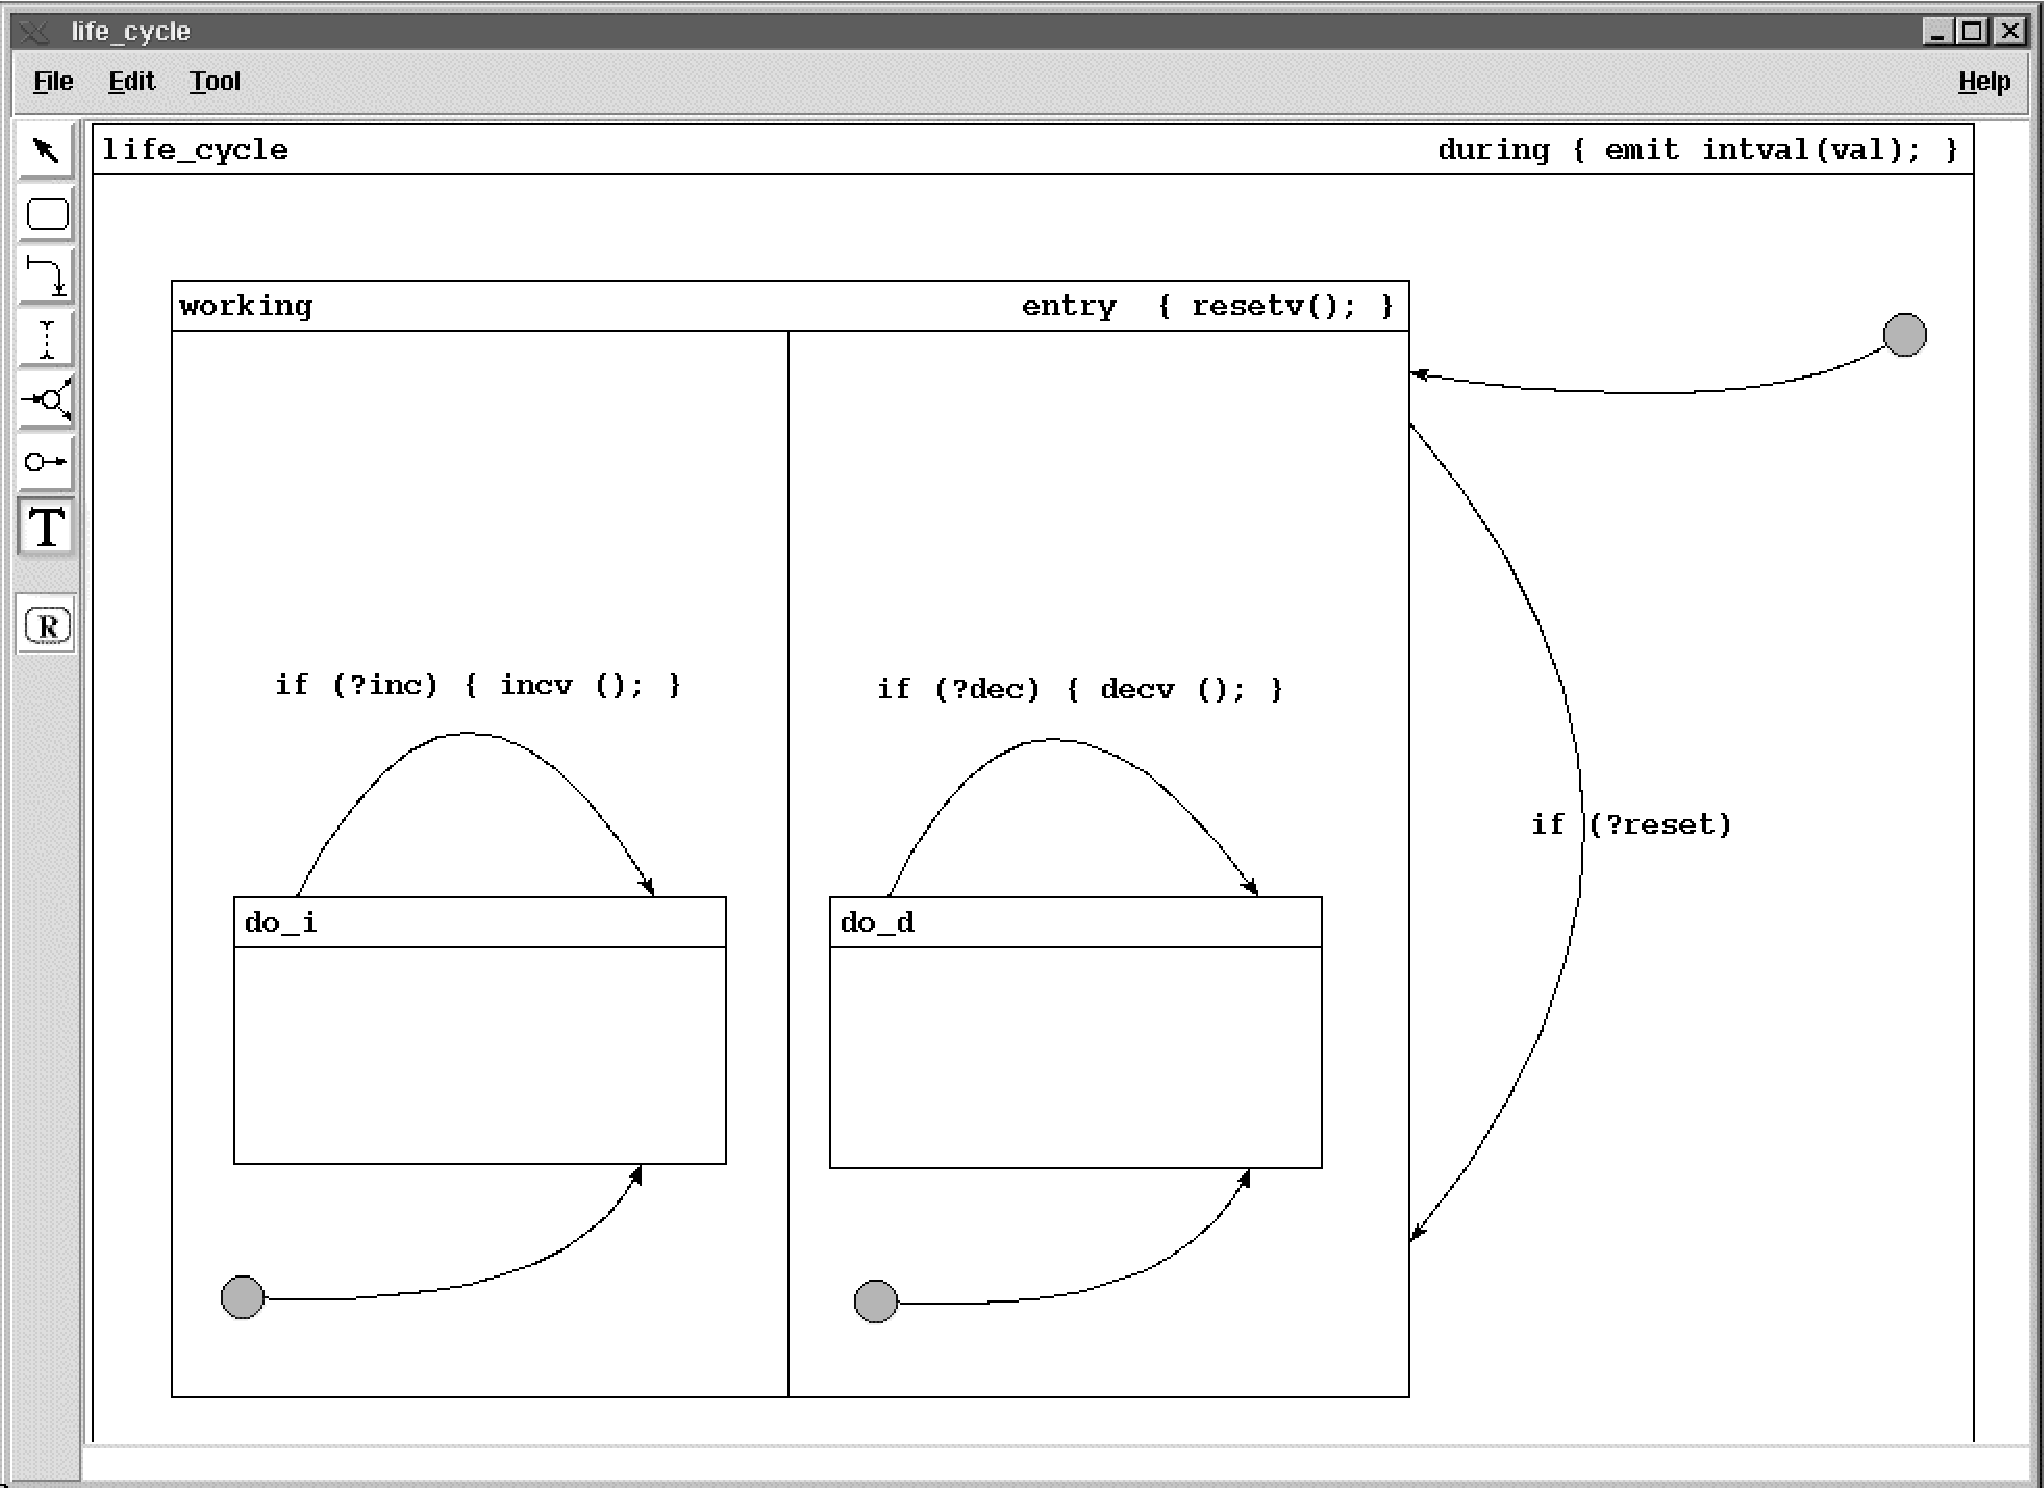
\includegraphics[width=250pt]{../pdf/incdec}
\end{center}

{\em
\section{\it Approximating \statecharts\ Semantics.}\index{Statecharts!semantics}

Emittance of signals is always delayed in \statecharts. Hence delayed signals as introduced in Section~\ref{reactive-control} may be used to approximate the \statecharts\ semantics.

There has been a certain amount of discussion whether the statecharts interpretation is truely synchronous. Rather than to join the flame, we believe that both signals and delayed signals have their merits and their shortcomings. Delayed signals cut causality cycles but a ``reaction'' may take more than one instant. The delays caused by delayed signals may be difficult to compute. Consider, for example, the familiar four bit counter but replacing signals by delayed signals.
% 
\codeinput{delayed-four-bit-automaton}
% 
Let us assume that we are in the states \emph{\pp{up1}} and \emph{\pp{up2}}, and let \emph{\pp{incr}} be present.  Then \emph{\pp{carry}} is emitted for the next
instant, and the first subautomaton moves to the state \emph{\pp{down1}}.  In
the next instant, the signal \emph{\pp{carry}} is present, the state of the
second subautomaton is change to \emph{\pp{down2}}, and the signal \emph{\pp{reset}} is emitted for the next instant.  At the same instant \emph{\pp{incr}} may be present causing a move to state \\emph{pp{up1}}. Now in the next instant, the signal  \emph{\pp{reset}} is present, the signal  \emph{\pp{elapsed}} is emitted for  the next instant, and toplevel automaton moves to state \emph{\pp{off}}. 

Of course, the process does not behave like a counter. We like to stress that the behaviour is not so easy to trace if delayed signals are involved, the main disadvantage being that mistakes will only show at run time.
}

\section{Examples}

\subsection{The Stopwatch using Automaton}\label{stopwatch-automaon}

\paragraph{The simple stopwatch.}
We distinguish two states: the stopwatch being running, and the stopwatch being stopped. The stopwatch toggles between the states if the button \pp{start\_stop} is pressed.
% 
\codeinput{simple-stopwatch-automaton}
%
One should note a distinction to the stopwatch as defined in Section \ref{stopwatch}. Since preemption is weak the elapsed time is emitted if the signal \pp{start\_stop} is present in state \pp{running}. It is a design choice whether this should be the case or not. For the latter, we must use strong preemption.


\paragraph{The general stopwatch}
Analysing the general stopwatch of Section \ref{stopwatch} we realise that there are two states corresponding to the simple stopwatch, a further toggle between the \pp{running} state, and a state for reset. These are used in the automaton below
% 
\codeinput{stopwatch-general-automaton}
%
One should note that -- quite unlike to the approach using the ``imperative'' sublanguage -- designing in terms of automata ask for finding states. It seems that in case of the general stopwatch this results in a much clearer design. The transitions between the states are obvious. however, the same remark applies as in case of the simple stopwatch above in that only weak preemption is used that results in a slightly different behaviour that that of the original stopwatch.



%\subsection{Another Lift Example}

%\subsection{A Telephone Answering Machine}
%


